\documentclass[11pt]{article}   % list options between brackets
\usepackage{graphicx}  % most common package for figure handling
\usepackage{amsmath}  
\usepackage{amssymb}
\usepackage{url}
\usepackage{verbatim} % useful for displaying computer code or similar verbatim
\usepackage{full page} % This package changes the otherwise very generous margins to 1 inch on all sides
\usepackage{float}
\usepackage{listings}
\usepackage{amsmath}
\usepackage{changepage}
\usepackage{bigstrut}
\usepackage{rotating}
\usepackage{hyperref}
\usepackage{pdflscape }
\usepackage{program}
\usepackage[framed,numbered,autolinebreaks,useliterate]{mcode}

 \usepackage{algpseudocode}
\usepackage{subfig}
\begin{document}
\setlength{\parindent}{0.00in}
%\ttfamily

\title{EN2202 Assignment 2}

\author{
 Sam Lewis\\
 svrlewis@kth.se
  \and
  Bjoern Fischer  
}
\date{} 
\maketitle
\linespread{1.5}

\section{Plots of the sound signals over the time domain}

The female speech signal was plotted and sections of the signal were examined to find the oscillitory behavior of voiced segments and the noisy behaviour of unvoiced segments. The code that was used to create these plots can be found in \texttt{timePlots.m}.

\begin{figure}[H]
\begin{center}
\leavevmode
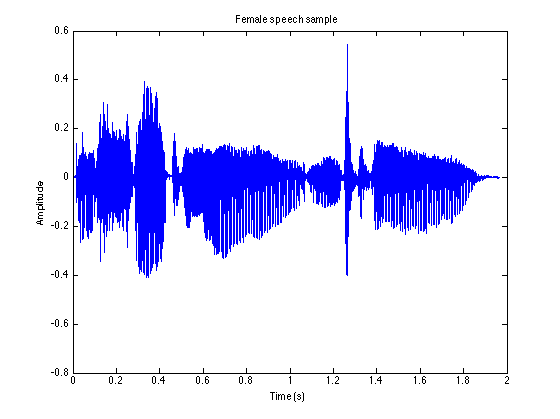
\includegraphics[width=0.75\textwidth]{female.png}
\end{center}
\caption{The complete female speech signal}
\label{euler:1}
\end{figure}


\newpage
The voiced sections of the signal were able to be located by looking for sections of the system that were oscillitory in nature - with some sort of repitition.

\begin{figure}[H]
\begin{center}
\leavevmode
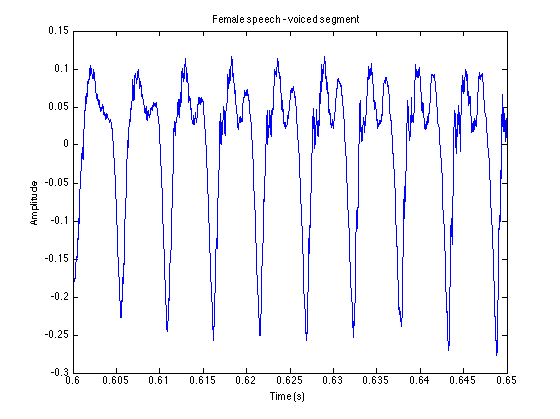
\includegraphics[width=0.6\textwidth]{voiced.png}
\end{center}
\caption{A voiced section of the female speech signal}
\label{euler:1}
\end{figure}

The unvoiced sections were then found by looking for noisy sections without any sort of pattern.

\begin{figure}[H]
\begin{center}
\leavevmode
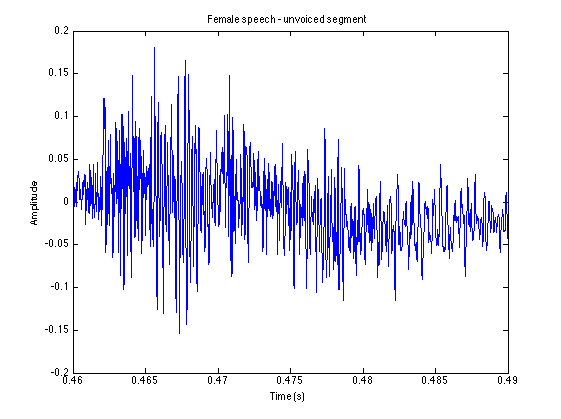
\includegraphics[width=0.6\textwidth]{unvoiced.png}
\end{center}
\caption{An unvoiced section of the female speech signal}
\label{euler:1}
\end{figure}

Finally, the music signal was also plotted.

\begin{figure}[H]
\begin{center}
\leavevmode
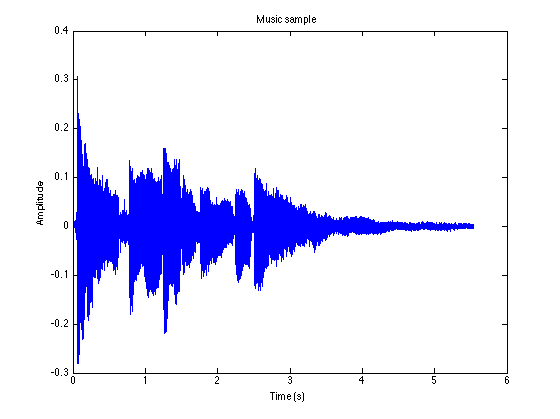
\includegraphics[width=0.6\textwidth]{music.png}
\end{center}
\caption{The complete music signal}
\label{euler:1}
\end{figure}

\newpage
\section{Spectrograms}

Spectrograms for the two signals shown previously were also plotted. For the music signal, harmonics representing the music sample were highlighted.

\begin{figure}[H]
\begin{center}
\leavevmode
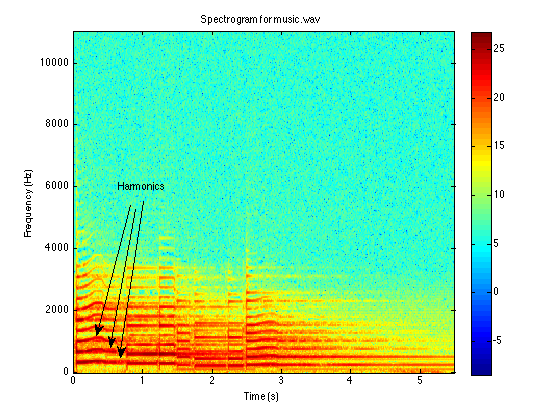
\includegraphics[width=1\textwidth]{musicspect.png}
\end{center}
\caption{Spectrogram for the music speech signal}
\label{euler:1}
\end{figure}

For the female speech sample, it was possible to locate the segments of voice  by looking for areas in the spectrogram where there were harmonics. On the other hand, segments of unvoice were obvious from the areas in the spectrogram where there was no pattern in the frequency distribution. One voice segment and one unvoiced segment were highlighted on the diagram as seen below. 


\begin{figure}[H]
\begin{center}
\leavevmode
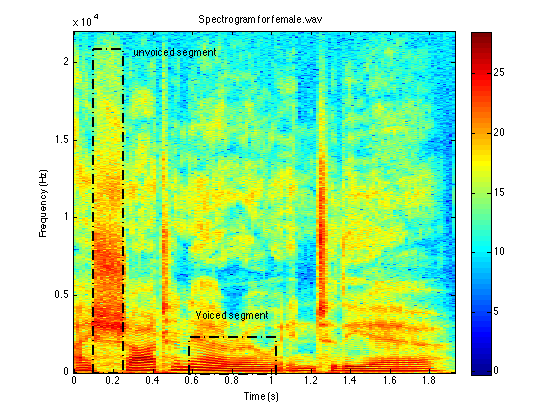
\includegraphics[width=1\textwidth]{femspect.png}
\end{center}
\caption{Spectrogram for the music speech signal}
\label{euler:1}
\end{figure}

The code used to create these plots can be found in \texttt{spectrogram.m}

\newpage

\section{Cepstrograms}

Normalised cepstrograms were also found and then plotted, alongside the spectrograms for the three different signals. The figure below shows the spectrogram and cepstrogram for the music file. 

\begin{figure}[H]
\begin{center}
\leavevmode
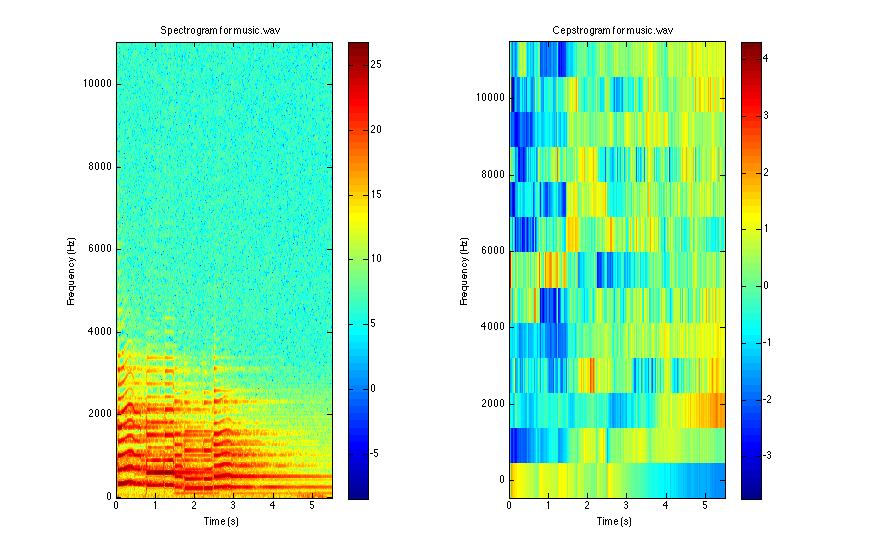
\includegraphics[width=1\textwidth]{musicCepstro.png}
\end{center}
\caption{Spectrogram and cepstrogram for the music speech signal}
\label{euler:1}
\end{figure}

\newpage
Then, to analyse the differences between a male and female speaking the same phrase, the spectrogram and cepstrogram of the male and female speech samples were plotted together. The script to create these plots is \texttt{cepstrograms.m}.


\begin{figure}[H]
\begin{center}
\leavevmode
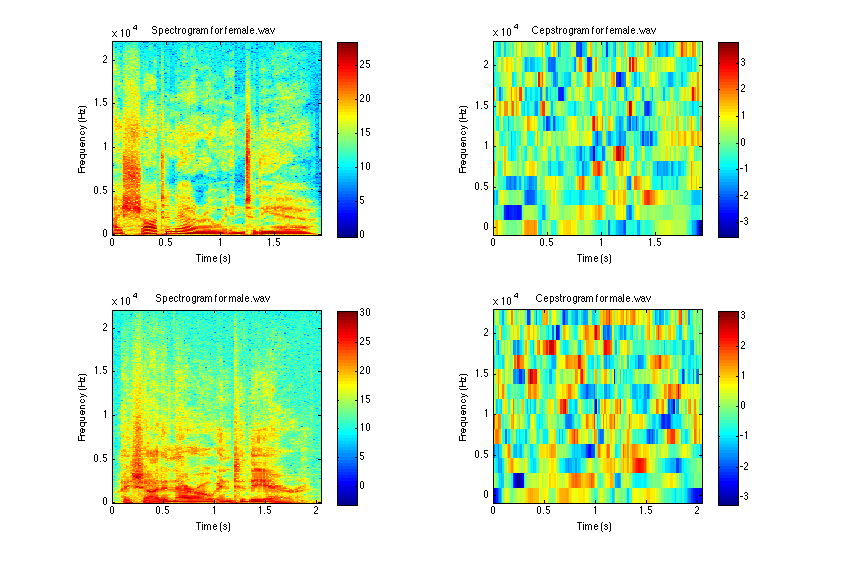
\includegraphics[width=1\textwidth]{speechCepstro.png}
\end{center}
\caption{Spectrogram and cepstogram for the male and female speech signals}
\label{euler:1}
\end{figure}

\newpage

\section{Correlation matrices}

For the female speech sample, the correlation matrices for the spectral and cepstral coeffecient series were found. The MATLAB code used to create these plots is in \texttt{correlation.m}.


\begin{figure}[H]
\begin{center}
\leavevmode
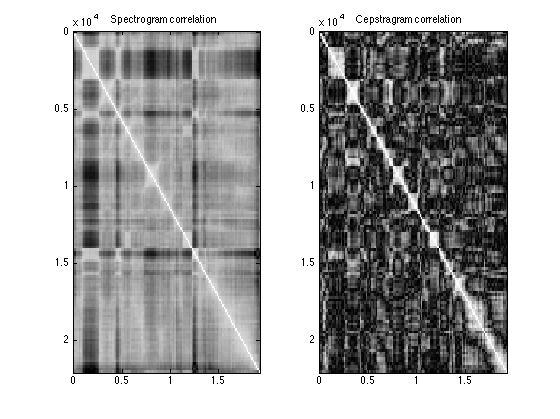
\includegraphics[width=1\textwidth]{corr.png}
\end{center}
\caption{Spectrogram and cepstogram for the male and female speech signals}
\label{euler:1}
\end{figure}

\newpage

\section{Questions}
\textit{Which reprsentaton do you think is easiest for you, as a human, to interpret, and why?}\\

\begin{adjustwidth}{2.5em}{0pt}
Personally, for me, the spectrogram is much easier to interpret. As a human it is easier to filter the information and have an idea about the general trend of the signal so that, for example, it is possible to interpret when there are sections of voice or unvoice. The spectrogram is not as easy to understand and looks a lot more unorganised.
\end{adjustwidth}\

\textit{Can you see that the spectrograms represent the same phrase? Could a computer discover this?}\\

\begin{adjustwidth}{2.5em}{0pt}
Comparing the male and female spectrograms for the same phrase, it is possible to find the similarities and see that certain sounds, though they may be said with slight differences because of the gender and individual accents of the speaker, are in the same order. \\

However, doing this sort of recognition would be hard for a computer as there is no mathematical rigour in comparing the two septrograms. More processing would need to be done.

\end{adjustwidth}\

\textit{Can you see that the cepstrograms represent the same phrase? What about a computer?}\\

\begin{adjustwidth}{2.5em}{0pt}
Comparing cepstrograms is much harder for me as it is harder to spot patterns. However, presenting the information in this way might make it easier for a computer to view how similar the signals are. This is because the information is more clearly broken up into chunks.
\end{adjustwidth}\

\textit{Which matrix, spectral or cepstral, looks the most diagonal?}\\

\begin{adjustwidth}{2.5em}{0pt}
Looking at the plots in figure 9, the cepstrogram looks the most diagonal. This is as the areas outside the diagonal are darker than in the correlation of the spectrogram, meaning the intensity outside of the diagonal is weaker.

\end{adjustwidth}\

\textit{How could a MFCC represenation in a speech recognizer be confused?}\\

\begin{adjustwidth}{2.5em}{0pt}
To improve the performance in pattern recognition for speech recognition, the pitch of the signal is removed. Although pitch is not important in the recognition of individual words, it still carries important information in complete phrases. For example, the phrase 'you are an engineer' in English can be both a question or a statement depending on the intonation. Because the pitch of the words in the phrase are discarded in the speech recognition system, it would not be possible to find the meaning of the phrase. \\

On the other hand, there may be cases where the accent of a person or a speech impediment would make the phrase from a person seem different than the same phrase from another person for a MFCC but not for a human.\end{adjustwidth}\

\end{document}


